\chapter{Introducing MATSim}
\label{ch:introducing}
% ##################################################################################################################
\hfill \textbf{Author:} Andreas Horni, Kai Nagel, Kay W. Axhausen

\begin{center} 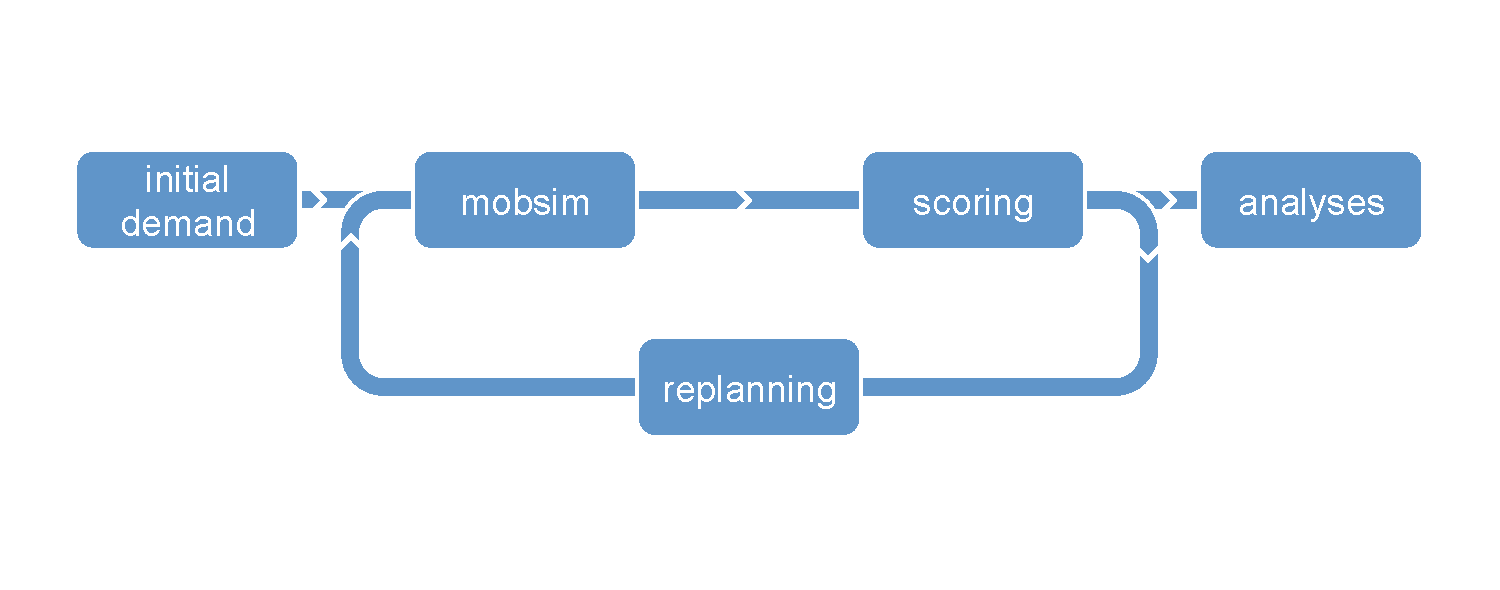
\includegraphics[width=0.7\textwidth, angle=0]{figures/matsimcycle.pdf} \end{center}

% ##################################################################################################################
\section{The Beginnings}
\label{sec:howitstarted}
The \gls{matsim} project \citep[][]{MATSIM_Webpage_2015} started with the wish of Kai~Nagel, then at ETH Zürich, to improve on his work with and for the \gls{transims} project \citep[][]{SmithEtc1995TRANSIMSSeattle,TRANSIMSFHWA_Webpage_2013} and to make the resulting code open-source.\footnote{%
%
TRANSIMS has since then also become open source \citep{TRANSIMSOS_Webpage_2013}, but around 2000 TRANSIMS was difficult to procure in Europe.
%
} After Kai~Nagel's departure to Berlin in 2004, Kay~W.~Axhausen joined the effort in earnest. A collaboration---successful and productive since more than 10\,years ago---was thereby established, combining the physicist's and the civil engineer's perspective, and bringing together expertise in
%
traffic flow,
%
\gls{largescale} computation,
%
choice modeling,
%
and
%
\gls{cas}:
%
%% \st{His background in traffic flow, complex adaptive systems, and large-scale computation was complemented with experience in the agent-based modeling of travel demand when---after Kai~Nagel's departure to Berlin in 2004---Kay~W.~Axhausen joined the effort in earnest.}
%
%% \ah{Transims war doch auch schon agent-based, oder?}
%
%% \kai{Transims hatte individuelle Personen mit Plänen für Aktivitäten und Routen.  Aber die Information war über mehrere Dateien verteilt: eine für die synthetic population, eine für die activity plans, eine für die trips.  Als Resultat hatte die dynamische Umlegung z.B.\ nicht das Einkommen der Person, oder der zweite Trip eines Agenten konnte starten, bevor der erste beendet war. -- Daher war es wohl ``weniger'' agenten-orientiert als matsim.}
%
%% \st{It is this merger of two, actually three large and old streams of research, which has made the system unique from the start:}
%
%% \ah{Gilt das genauso für Transims (?), so unique war das also auf dieser Ebene beim Start nicht oder? Die Unterschiede sind eher bei "MATSim had to important differences..." (siehe unten)}
%% \ah{unique? Wie genau hängt dies mit den Strands unten zusammen. Dem Leser Zusammenhang zeigen. Reihenfolge ändern 1 $\to$ 2 ?}
%
%% \ah{transition}
%
%% As detailed in Chapter~\ref{ch:history}, about \gls{matsim}'s history, \gls{matsim} 
%% %is a merger of three large and old 
%% combines several streams of research, namely 
\begin{itemize}\styleItemize
%
\item \textbf{Microscopic modeling of traffic:} \gls{matsim} performs integral microscopic \emph{simulation of the resulting traffic flows} and the resulting congestion (see Section~\ref{sec:trafficflowmodel}).
%
\item \textbf{Microscopic behavioral modeling of demand/agent-based modeling:}
%\textbf{Agent-Based Modeling:} 
  \gls{matsim} uses a microscopic description of demand by \emph{tracing the daily schedule} and the decisions involved of the synthetic travelers.  This may be called ``agent-based'' in retrospect.
  %% \ah{Könnte man das agent-based modeling mit ``...''/ in den Bullet-Titel nehmen, wie mal als Vorschlag eingefügt? Ist ja ein zentraler Begriff für MATSim.}
  % ok.  kai, jan'15
%
\item \textbf{Computational physics:}
%% , in particular simple and thereby fast models of physical processes:} 
%% Computational physics has performed simulations with $10^8$ and more particles already in the 1980s.
\gls{matsim} performs fast microscopic simulations with $10^7$ or more ``particles''.
%
\item  \textbf{Complex adaptive systems/co-evolutionary algorithms:}
 %% and equilibrium modeling:} 
\gls{matsim} \emph{optimizes the experienced utilities} of the whole schedule through the co-evolutionary search for the resulting equilibrium or steady state (see Section~\ref{sec:co-ev}). 
%
%% \kai{Andreas, habe ``equilibrium modelling'' aus der Überschrift rausgenommen.  Ist das für irgendwen wichtig? Für mich war/ist equilibrium immer nur eine Krücke.  Eigentlich ist auch hier das entscheidende Paper \citep{ArthurBar}, welches gerade darauf hinausläuft, dass man ``coordination'' auch bekommt, ohne dass die Agenten ökonometrisch optimieren.}

\end{itemize}

%\kai{Habe an obigem nochmal rumgeschrieben. Nachdem ich die ``bullets'' dann fertig hatte, sahen sie fast genauso aus wie die bereits vorher existierende Aufzählung nach ``bringing together expertise''.}

%% \ah{changed order to make it consistent with order below (now in history)}

%% \st{The robustness of this framework for the description of all congested spatial behaviors became clear as the development progressed to include the congestion inside facilities and buildings or as parking was added.} \ah{etwas weg von Argumentationslinie?}

%% \ah{moved everything from here to history}

%In transport modeling, these streams have evolved from the 1970's for microscopic traffic flow and agent-based demand modeling \citep[e.g.,][]{Wiedemann_PhDThesis_1974, Seddon_Simulation_1972}, while transport equilibrium modeling already started in the 1950's \citep[][]{Wardrop_PICE_1952}. At the end of 1990’s the scene was set for a merger of these strands into a computationally efficient, modular and open-source software enabling further development on travel behavior, network response and efficient computation: \gls{matsim}.

At the end of 1990’s the scene was set for these research streams' merger into a computationally efficient, modular and open-source software enabling further development on travel behavior, network response and efficient computation: \gls{matsim}.

% ----------------------------

%\ah{alles ab hier würde ich viel lieber in Chapter~\ref{ch:history} sehen. Hier will man doch nur ein Häppchen History um MATSim grob einordnen zu können. Ohne breites Hintergrundwissen sind nachfolgende Abschnitte nicht leicht verdaubar.}
%\ah{Würde hier einfach noch 2,3 Sätze in Richtung ... merging microscopic modeling, the agent-based approach and the notion of equilibrium ... usw.}
%\ah{und dann enden mit "At the end of 1990’s the scene was set for a merger of these strands into a computationally efficient, modular and open-source software enabling further development on travel behavior, network response and efficient computation."}
%\ah{Was meinst du? Könnte das sonst mal versuchen ...}
%\kai{Von mir aus sehr gerne.}

% ----------------------------

%% As shown on the web page \citet[][]{MATSIM-Scenarios_Webpage_2015} and detailed in Chapter \ref{ch:scenarios}, \gls{matsim} has been applied by local research groups world-wide for multiple different regions. 
%% % \ah{see Discussion~\ref{sec:matsimtd}}
%
%finde den jetzt auskommentierten Absatz arg ``out of context''.  M.E. müsste da entweder zusätzliches Text drumrum, oder wir lassen ihn weg.  Habe ihn jetzt erstmal auskommentiert.  kai, dec'14

% ##################################################################################################################
\section{In Brief}
\label{sec:inbrief}
\gls{matsim} is an activity-based, extendable, multi-agent simulation \gls{framework} 
%toolkit
%\kai{m.E.\ framework} 
implemented with 
%the current version of 
\gls{java}. It is open-source and can be downloaded from the Internet \citep[][]{MATSIM_Webpage_2015, SourceForge_Webpage_2015}. The \gls{framework} is especially designed for large-scale scenarios, meaning that the features of all models are generally stripped down to efficiently handle the targeted functionality, where emphasis has been also been laid on parallelization \citep[e.g.,][]{Dobler_TechRep_IVT_2011, Charypar_PhDThesis_2008}. For the network loading simulation, for example, a queue-based model is implemented, leaving out the very complex and computationally expensive car-following behavior (see Section~\ref{sec:trafficflowmodel}).

For now, \gls{matsim} is 
%conceptually 
%
%I don't think it is ``conceptually''.  If anything, it is just the current software. kai, jan'15
designed to model a \emph{single day}, the common unit of analysis for \gls{activitybased} models (see, for example, the review in \citet[][]{Bowman_TEC_2009_1}). In other words, \gls{matsim} is limited to the dynamics within that day. Nevertheless, in principle a multi-day model could be implemented \citep[][]{ZilskeEtc2012AddingFreightToMatsim,HorniEtAl_TechRep_IVT_2012_a}.

As shown in Section~\ref{sec:co-ev}, \gls{matsim} is based on the co-evolutionary principle. While being in a competition for space-time slots on the transportation infrastructure with all the other agents, every agent repeatedly optimizes its daily \gls{activity} schedule.  This is a bit similar to the iterative cycle of route assignment, but goes beyond route assignment by including other choice dimensions such as time choice \citep{BalmerRaneyEtAl2005act-times}, mode choice \citep{GretherEtAl2009SimpleModeChoiceIPL}, or destination choice \citep{HorniEtAl2011TrbLocationChoice} into the iterative loop.
%% \kai{Andreas, fallen dir noch weitere Referenzen ein?} \ah{Ich würde sagen, dies ist die wichtigste.}

% ------------
%\begin{figure}
\createfigure%
{\protect\gls{matsim} loop, sometimes called the \protect\gls{matsim} cycle}%
{\protect\gls{matsim} loop, sometimes called the \protect\gls{matsim} cycle %% \kai{Andreas, I replaced ``execution'' by ``mobsim''.} \ah{perfect. I think, we have to do that at various other places on the webpage (?)}}%
  % oh well.  Konzentrieren wir uns erstmal auf das Buch, und darauf, dass die URLs im Buch sinnvoll und stabil sind. kai, jan'15
%, sometimes also called the "MATSim washing machine"}%
}
{\label{fig:matsimcycle}}%
{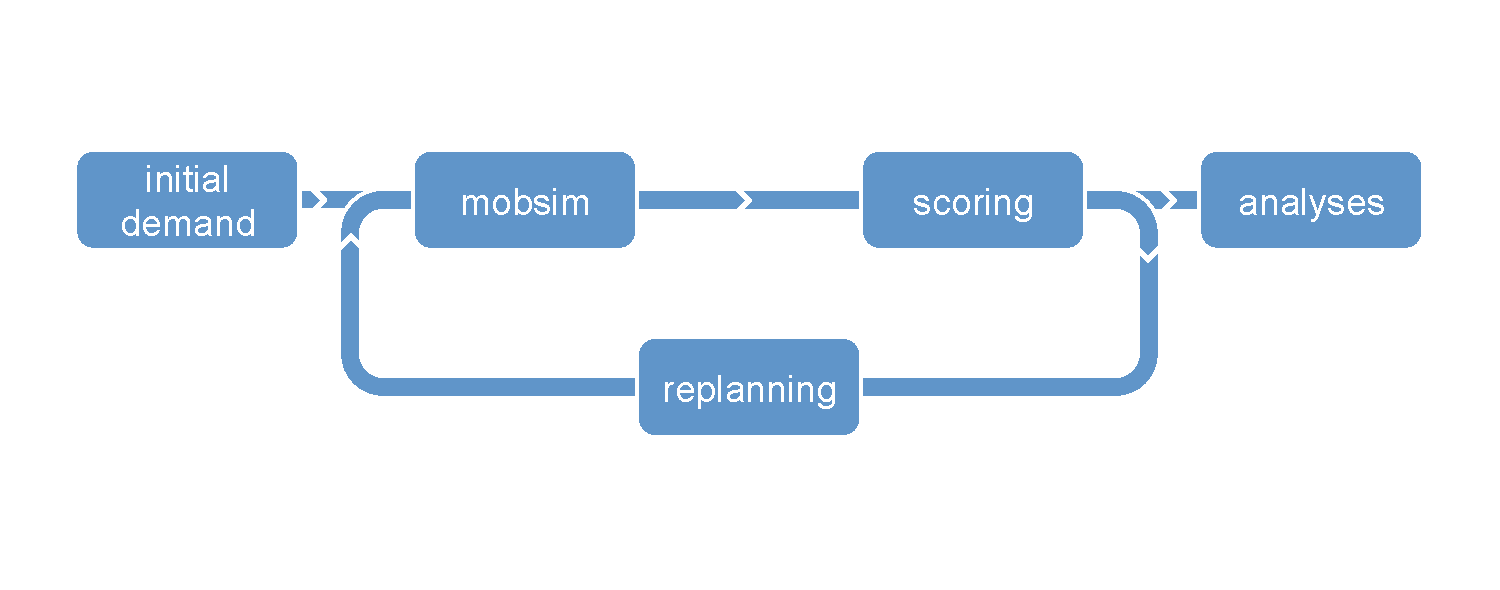
\includegraphics[width=0.99\textwidth, angle=0]{figures/matsimcycle.pdf}}%
{}
%\end{figure}
% ------------

A \gls{matsimrun} contains a configurable number of iterations represented by the loop of Figure~\ref{fig:matsimcycle} and detailed below. 
%
It starts with an initial demand, which arises from the \gls{study} area population's daily activity chains. The modeled persons are called agents in \gls{matsim}. The activity chains are usually derived from empirical data through sampling or discrete choice modeling. A variety of approaches is suitable as can be seen in the scenarios' chapter (Chapter~\ref{ch:scenarios}). During the iterations this initial demand is optimized. Every agent possesses a memory of a fixed number of day plans, where each \gls{plan} is composed of a daily activity chain and an associated \gls{score}.  The score can have an interpretation as econometric utility (\cf Chapter~\ref{ch:economicEval}).

In every iteration, prior to the simulation of the network loading with the \gls{matsim} \emph{\gls{mobsim}} \citep[e.g.,][]{Cetin_PhDThesis_2005}, every agent selects a plan from its memory. This selection is dependent on the plan \emph{scores}, which are computed after each mobsim run, based on the executed plans' performances. A certain share of the agents 
%$\varphi$ 
(often 10\,\%) is allowed to clone the selected plan and modify this clone (\emph{\gls{replanning}}).
%% With the \gls{msa} usually a decreasing share of travelers is reallocated to a new plan to avoid oscillations. For \gls{matsim}, it has been shown that a variable replanning share over the course of the iterations can be productive and \emph{"increases overall performance of the system by a factor of three or more"} \citep[][p.7f]{CharyparEtAl_IATBR_2006}.
%% \kai{Andreas, ich habe das mit dem ``decreasing share of travelers'' mal rausgenommen.  M.E.\ ist das weder im core noch in einer contrib implementiert.  Somit gehört es auf jeden Fall nicht nach ``using matsim''.  --  Es gibt einen MSA switch, aber der bezieht sich auf den score. --  Falls die Aussagen von DC im Buch vorkommen sollen, müssten sie wohl eher irgendwo nach ``understanding matsim''.} \ah{Danke!}
For the network loading 
%microsimulation % \ah{to me microsimulation is not a necessary word hier.}
step, multiple \glspl{mobsim} are available and configurable \citep[][p.10f]{HorniEtAl_TechRep_IVT_2011_a, MATSim_Userguide_2015}. 

Plan modification is performed by the \emph{replanning} modules. Four dimensions are usually considered for \gls{matsim} at this time: departure time (and implicitly activity duration) \citep[][]{BalmerRaneyEtAl2005act-times}, route \citep[]{LefebvreBalmer_STRC_2007}, mode \citep{GretherEtAl2009SimpleModeChoiceIPL}, and destination \citep{HorniEtc2008locachoice,HorniEtAl2011TrbLocationChoice}. Further dimensions such as activity adding or dropping or parking and group choices are currently under development and only available experimentally. % Siehe Tabelle MATSim-Präsentationen Prof.\ Axhausen.
\gls{matsim} replanning offers different strategies to adapt plans ranging from random mutation to approximate suggestions, to best response answers where in every iteration the currently optimal choice is searched. For example, routing
%and destination replanning are
often is a best response modification%
%(possibly taking into account ``frozen'' randomness)
, while time and mode replanning are random mutations.
%% \kai{Andreas, habe in obigem Satz locachoice rausgenommen.  (1) Echte best response ist m.E.\ technisch schwierig, weil der router nicht die genauen Reisezeiten ausspuckt.  Thibaut sieht das m.E.\ genauso.  (2) Wenn Du tatsächlich echte best response machst, dann müsste doch immer das gleiche rauskommen, es sei denn, die Reisezeiten ändern sich drastisch von einem Aufruf zum nächsten. -- Man könnte es reinnehmen, bräuchte dann aber m.E.\ auch einen Hinweis auf die frozen randomness, was für dieses frühe Kapitel vielleicht zu schwergewichtig daherkommt?} \ah{ok. Reine best response ist es ja sowieso nicht, weil ich um den Approximationsfehler im Back-wards Dijkstra zu kompensieren wieder Probs bei der provisorischen Auswahl reingenommen habe.}

The initial day chains do not need to be very carefully defined for the replanning dimensions that are included in the optimization process. Plausible values just speed-up the optimization process. 

If an agent ends up with too many plans (configurable), the plan with the lowest score (configurable) is removed from the memory of this agent. The agents that have not undergone replanning select between existing plans. The selection model is configurable; in many \gls{matsim} investigations, a model that generates a logit distribution for plan selection is used.

An iteration is completed by evaluating the agents' day experience of the selected day plans (\emph{scoring}). The applied scoring function is described in detail in Chapter \ref{ch:scoring}.

% ------------
\createfigure[t]%
{Typical score progress}%
{Typical score progress}%
{\label{fig:scoreprogress}}%
{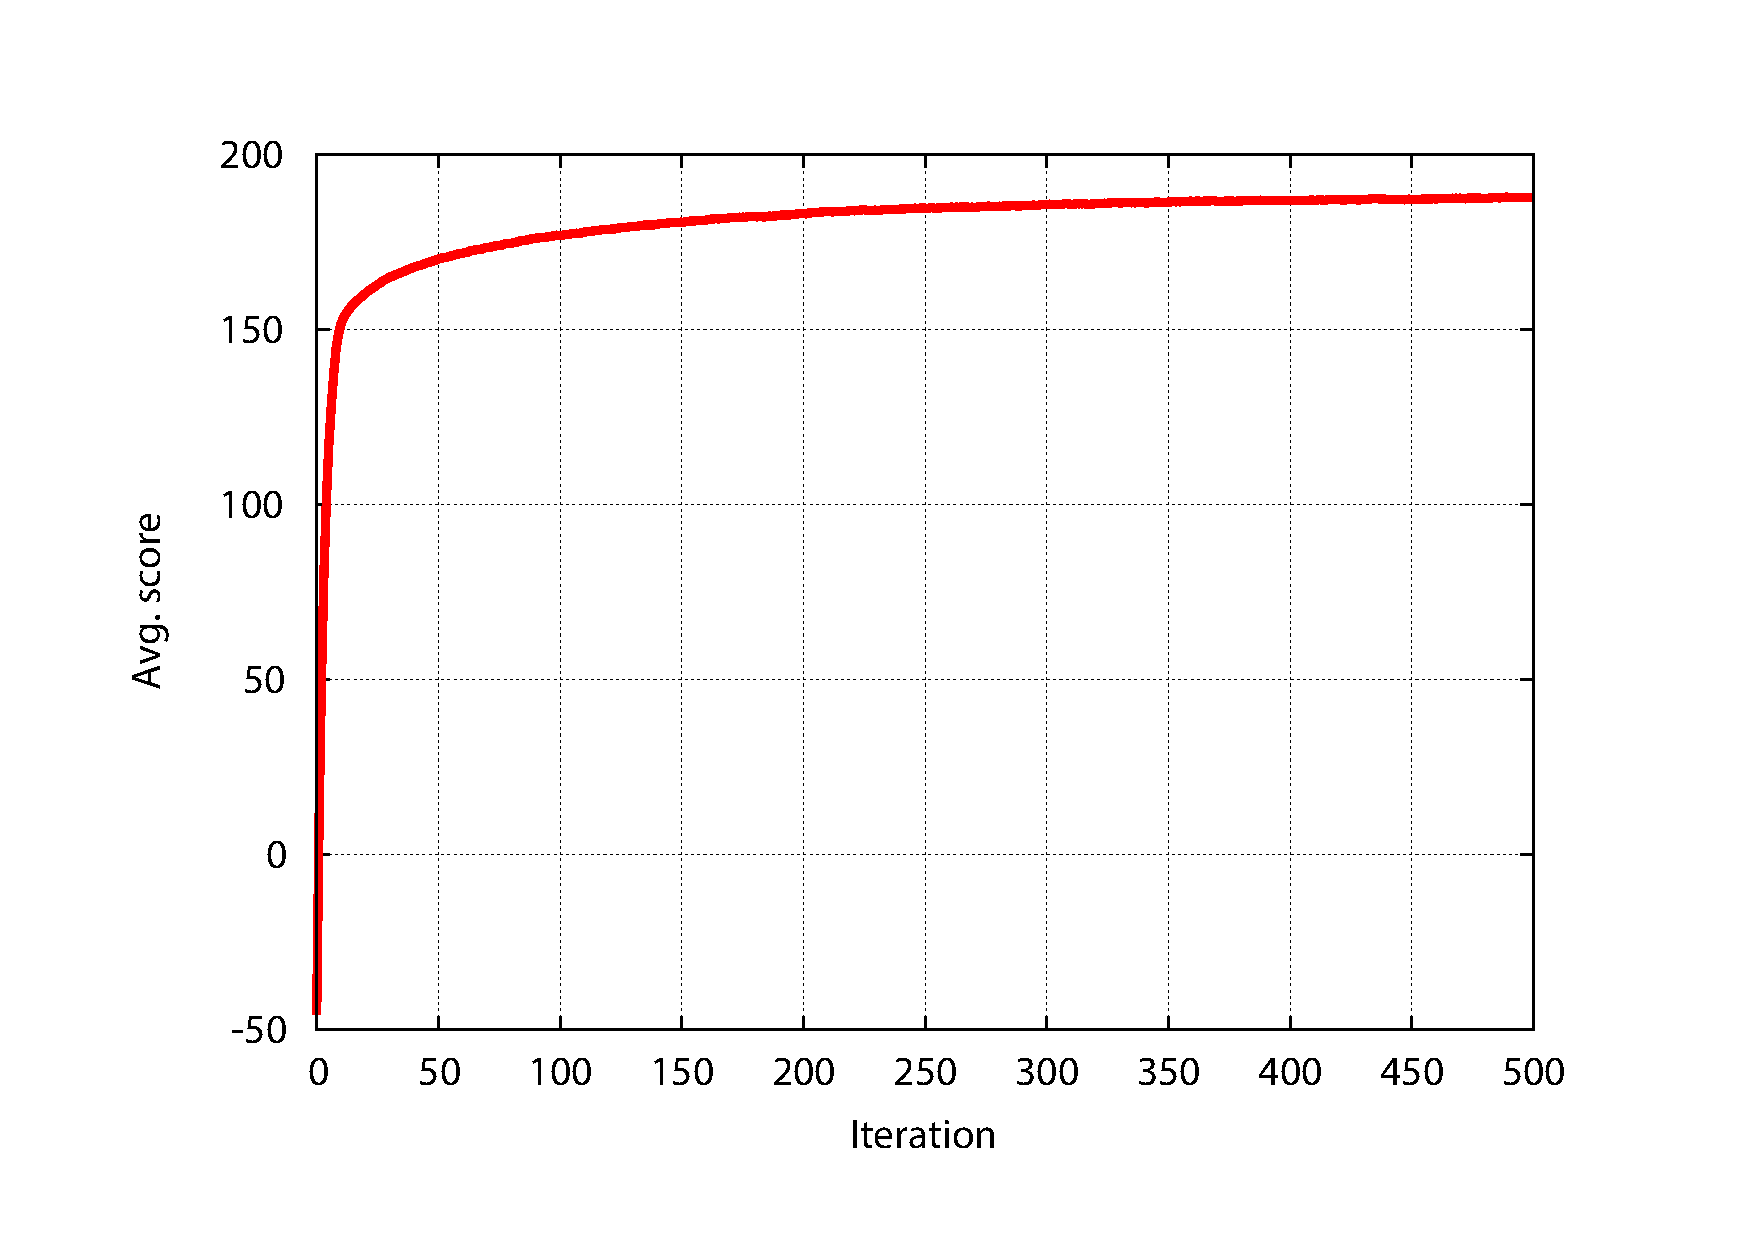
\includegraphics[width=0.99\textwidth, angle=0]{using/figures/scores.pdf}}%
{}
% ------------

The iterative process is repeated until the average population score stabilizes.
%% , where the definition of the stopping criterion is subject of research initialized by \citet[][]{Meister_PhDThesis_2011, NagelFloetteroed2009IatbrResourceInBook}.
The typical score development curve (Figure~\ref{fig:scoreprogress}, taken from \citet[][]{HorniEtAl_TRR_2009}) has the form of an evolutionary optimization progress \citep[][Figure~2.5]{EibenSmithJE_2003}.  Since the simulations are stochastic, it is not possible to use convergence criteria appropriate for deterministic algorithms; for a discussion of possible approaches for the \gls{matsim} situation see Chapters~\ref{sec:score-convergence} and \ref{sec:Relaxation-as-a} as well as \citet{Meister_PhDThesis_2011}.

\gls{matsim} offers considerable customizability through its modular design. Although %replacing
implementing alternative core modules, such as an alternative network loading simulation, may be associated with a substantial effort \citep[][Section 2.4]{MATSim_Userguide_2015}, in principle every module of the framework can be exchanged. \gls{matsim} modules are described in Chapter~\ref{ch:modules} and following.

\gls{matsim} is heavily based on events. Every action in the simulation generates an event, which is recorded for analysis. These event records can be aggregated to evaluate any measure at the desired resolution. The event architecture is detailed in Section~\ref{sec:events-extension-point}.

% ##################################################################################################################
\section{MATSim's Traffic Flow Model}
\label{sec:trafficflowmodel}
\gls{matsim} provides two internal \glspl{mobsim}: \gls{qsim} and \gls{jdeqsim}. Furthermore, external mobility simulations can be plugged in. Some years ago the \gls{deqsim} written in \gls{cpp} and described by \citet[][]{Charypar_PhDThesis_2008, CharyparEtAl_TRR_2007, CharyparEtAl_TRB_2009, CharyparEtAl_WCTRS_2007} was plugged into \gls{matsim} and frequently used. The multi-threaded \gls{qsim} is the default \gls{mobsim} \citep[][]{MATSim_Userguide_2015}. % commit 29999 michaz

\citet[][]{CharyparEtAl_TRB_2009} distinguishes between 
\begin{itemize}\styleItemize
\item physical simulations, featuring detailed car following models, %\ah{I have changed simulations for microsimulation}
\item cellular automata, in which roads are discretized into cells,
\item queue-based simulations, where traffic dynamics are modeled with waiting queues,
\item mesoscopic models, using aggregates to determine travel speeds, and
\item macroscopic models, based on flows rather than single traveler units (\eg cars).
\end{itemize}

As \gls{matsim} is designed for large-scale \glspl{scenario} it adopts the computationally efficient queue-based approach (see Figure~\ref{fig:queue}). A car entering a network link (\ie a road segment) is added to the tail of the waiting queue. It remains there until the time for traveling the link with free flow has passed and until he or she is the head of the waiting queue and until the next destination link allows entering. The approach is very efficient, but clearly it comes at the price of reduced resolution, \ie car following effects are not captured.   
%
\createfigure%
{Traffic flow model}%
{Traffic flow model}%
{\label{fig:queue}}%
{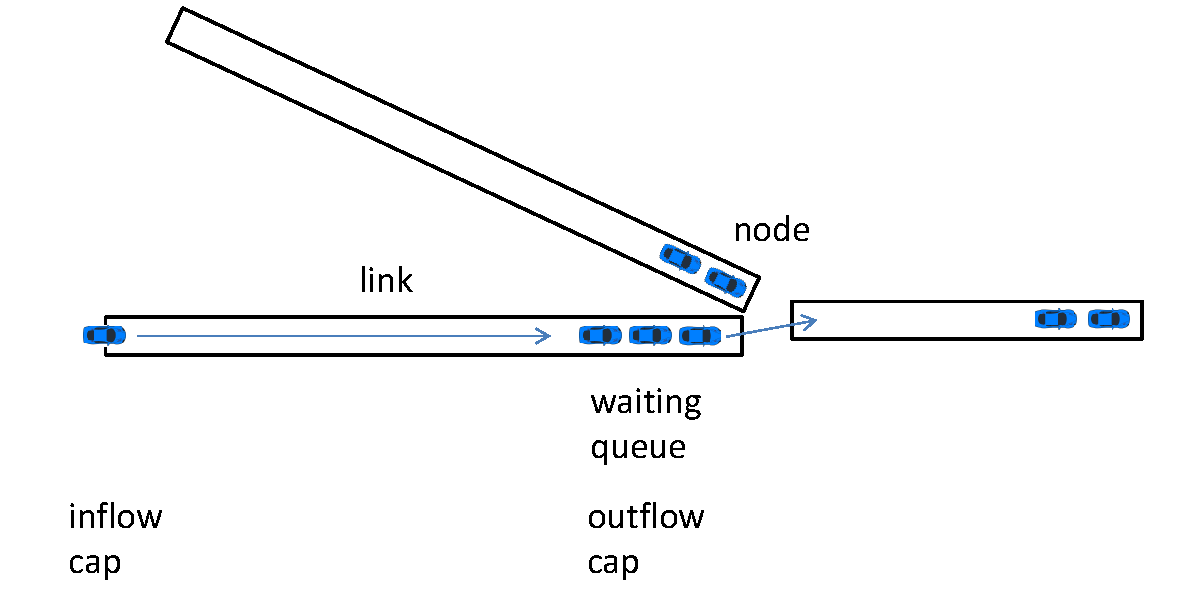
\includegraphics[width=0.9\textwidth, angle=0]{using/figures/queue.pdf}}%
{}
%
In \gls{jdeqsim}, for computational reasons the waiting-queue approach is combined with an event-based update step \citep[][]{CharyparEtAl_TRB_2009}. In other words, there is no time-step-based updating process of any agent in the scenario. Instead agents are only touched if they actually require an action. For example, links do not have to be processed while agents traverse them.
%% an agent needs to pass a link (i.e., he or she is waiting in the queue), he or she does not need to be processed.
%
%"and agent (that) needs to pass a link" wird auch in der normale QSim nicht angefasst.  ALLERDINGS fasst die normale QSim Kanten an, auf denen Agenten unterwegs sind ... selbst wenn wir wissen, dass sie frühestens in einer Stunde rauskommen können. kai, jan'2015
%
%\kai{Ich kriege Ärger, wenn agents immer nur männlich sind.  Ist kein Witz; wurde mir bei meinen ersten öffentlichen Auftritten in Berlin sehr deutlich bedeutet.}  
% \ah{korrigiert}
Triggering of update events is managed by a global scheduler. \gls{qsim}, however, is time-step based. 
%\ah{see Discussion~\ref{sec:scenariod}}
%
%\kai{Aber in der QSim ist das nicht so; die ist ganz normal time-stepped.  Sie schaltet nur Kanten ab, die nicht ``aktiv'' sind.} 
%
% \ah{korrigiert}
%
The \gls{matsim} traffic flow model is heavily based on the two attributes of a link: storage capacity and flow capacity. Storage capacity defines the number of cars fitting onto a network link.
%% It is a physical property and thus fixed in the simulation.
%
%% \kai{Andreas, I removed the statement ``it is a physical property and thus fixed in the simulation'' ... network change events können die Anzahl der Fahrspuren und damit die storage capacity verändern.} \ah{ok}
%
%% For scenarios with a population smaller then the full population, say a 10\% sample, however, it needs to be scaled down, since otherwise there will be no spill-back any more.

Flow capacity specifies the outflow capacity of a link, \ie how many travelers can leave the respective link. It is an individual attribute of the link. In the earlier \gls{deqsim} and in the current \gls{jdeqsim} an additional inflow capacity can be specified in addition to capture breakdowns at link entries \citep[][p.~99]{Charypar_PhDThesis_2008}. The many simulation experiments with \gls{qsim} (and the former queueSimulation) have shown that neglecting inflow capacity does not have a substantial effect but further reduces model complexity. 

This basic traffic flow model has been extended with various modules: signals and multiple lane modeling have been added (Chapter~\ref{ch:signalslanes}), backward-moving gaps as investigated by \citet[][]{Charypar_PhDThesis_2008} are included in \gls{jdeqsim} and available on an \emph{experimental base} for \gls{qsim}. 
Interactions between different modes are described in Chapter~\ref{ch:multimodalsim}. 
Limitations of the traffic flow model concern link dynamics (in particular overtaking and slow drivers) and intersection dynamics (in particular turn restrictions not explicitly modeled in the network). 


% ##################################################################################################################
\section{MATSim's Co-Evolutionary Algorithm}
\label{sec:co-ev}
%
% ------------
\createfigure[!h!t!]%
{The co-evolutionary algorithm in \protect\gls{matsim}}%
{The co-evolutionary algorithm in \protect\gls{matsim}
%
%% \kai{Andreas, warum ist beim allgemeinen co-evolutionary algorithm die interaction nicht bei der `fitness evaluation'?}
%% \ah{Mhhhm, Ort war abiträr gedacht, sollte einfach die Interaktion zwischen den Spezies zeigen. Habs jetzt raufgeschoben.}
%
}%
{\label{fig:ea}}%
{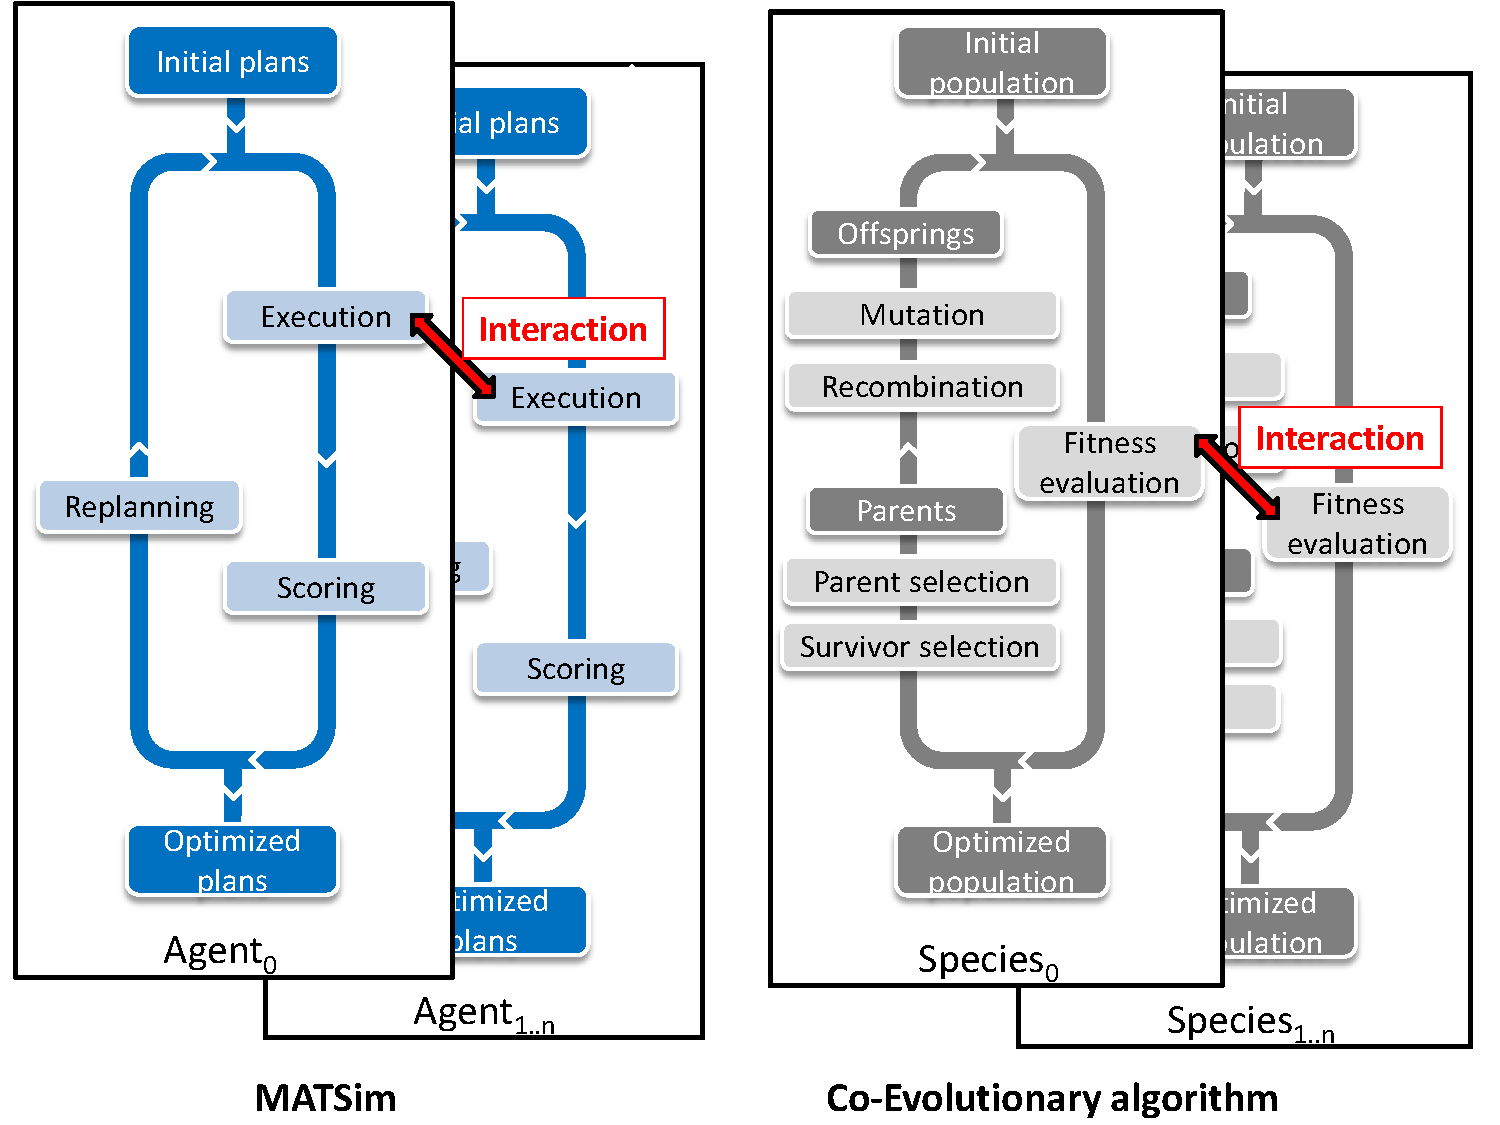
\includegraphics[width=0.99\textwidth, angle=0]{using/figures/MATSimVSea.pdf}}%
{}
% ------------
%
%\kai{Nett.  Gibt es eine Quelle für den ``co-evolutionary algorithm''?} \ah{fürs Bild? Hab ich mir selber aus den Fingern gesogen. Für Co-EAs allgemein?} \thibaut{du kannst \cite{PopoviciEtAl_2012} %gucken, find ich sehr gut. zum mindesten benutze ich immer diese in meine Papers}
%
As illustrated in Figure~\ref{fig:ea}, the \gls{matsim} equilibrium is searched by a \emph{\index{co-evolutionary algorithm}} \citep[see e.g.,][]{PopoviciEtAl_2012}. These \glspl{algorithm} co-evolve different species subject to interaction (\eg competition). In \gls{matsim}, the individuals are represented by their plans, where a person represents a species. With the co-evolutionary algorithm, optimization is performed in terms of agents' plans , \ie across the whole daily plan of activities and travel. It achieves more then the standard traffic flow \glspl{equilibrium}, which ignore the activities. Eventually, an equilibrium is reached subject to constraints, where the agents cannot further improve their plans unilaterally. 

%Strictly speaking, 
Note that there is a difference between application of an evolutionary algorithm and a \emph{co}-evolutionary algorithm. An evolutionary algorithm would lead to a system optimum as optimization is applied with a global (or population) fitness function. The co-evolutionary algorithm instead leads to a (stochastic) user \gls{equilibrium} as optimization is performed in terms of \emph{individual} scoring functions and within an agent's set of plans. 
%% At the moment, the \gls{matsim} co-evolutionary algorithm only includes mutation; recombination may come into play when coordinated day plans of family members, for example, are included in the future.
%
% einschränkende (und damit negative) Bemerkung, die m.E. an dieser Stelle nicht zwingend ist: genetische Algorithmen haben wohl etwas mit cross-over zu tun, evolutionäre (als Oberbegriff) aber nicht.  kai, jan'15

% ##################################################################################################################
%\section{Discussions}
% =============================================================================================
%\subsection{MATSim-T, MATSim-F, MATSim}
%\label{sec:matsimtd}
%
%\kai{Wie gesagt, ich wäre gegen ``MATSim-T'' und für einfach nur ``MATSim''.  Siehe \url{http://matsim.org/conceptual-meeting/2012/notes}.}
%
%\kai{
%Bei einem der meetings (m.E. conceptual, aber es mach auch developer gewesen sein) gab es mal eine Diskussion, ob wir die Bezeichnung "toolbox" wirklich beibehalten wollen.
%
%Wir waren uns damals einig, dass matsim eher ein framework als eine toolbox ist.
%
%(ca. 30 vs. ca. 3 hits auf matsim.org)
%
%Inzwischen, mit den "scripts-in-java", weicht das langsam ein wenig auf.  Aber wir hatten damals eigentlich beschlossen, sowohl auf "-T" als auch auf "-F" zu verzichten.
%
%(Wir brauchen einen "Stadtschreiber", damit wir uns an solche Diskussionen erinnern. :-) )
%
%Sollten wir das dann nicht auch im "Buch" machen?  Gibt es Personen, die an dem "-T" hängen?
%
%}
%
%\ah{erledigt}

% =============================================================================================
%\subsection{Scenario}
%\label{sec:scenariod}
%\kwaah{We should add at the start that 'scenario' is the combination of case study data (population size, initial plans, networks and facilities), policies, the selected replanning modules and the selected traffic flow simulation.} 
%
%\kai{I have to admit that I have that differently in my head.  
%%
%In the code, scenario is only the first, and this is also how I always had it in my own head: The ``XXX'' scenario is a collection of files.  
%%
%Selected \gls{replanning} \glspl{module} and selected traffic flow simulation is config; a sceanrio preferably comes together with a config that makes it runnable, but it is a different thing.  
%%
%And policy is policy; essentially the difference between (base case scenario | base case config) and (policy case scenario | policy case config).  
%%
%All three things together are a study for me.} 
%
%
%\kai{Wobei ``scenario'' so wie hier im ursprünglichen Text benutzt m.E.\ stehen bleiben kann.}
%%
%
%\kwaah{
%Kai, 
%
%I have no problem either way, but see many text where the inclusive use is implied. 
%
%But i am happy to see it split into 
%
%Scenario: population plans networks facilities
%
%Config = modules switched on
%
%Policies
%
%It is just that in many contexts in planning "Scenario" is equal to experiment or run. If we are consistent fine
%
%Kay
%}
%
%\kai{
%oh weh.  So etwas wie "the considered policy scenario is the large-scale introduction of autonomous vehicles in Los Angeles County"? 
%
%Vielleicht können wir 
%
%(1) versuchen, "policy scenario" und "(matsim) scenario" erstmal auseinander zu halten
%
%(2) es im Auge zu behalten, ob uns eine bessere Lösung einfällt.
%%
%...
%%
%Ich lese übrigens gerade nochmal (kleine) Teile des (großen) Buches von Russell/Norvig (Introduction to AI, a modern approach).  Da gibt es "utility based agents" ... 
%
%... aber "An agent's utility function is essentially an internalization of the performance measure."
%
%\textbf{\textit{Hier ist als "utility" nicht gleich "econometric utility"}}.
%}
%
%
%\kai{
%Im Satz davor:
%
%"a \textbf{performance measure} assigns a \textbf{score} to any given sequence of environment states"
%
%Ein Unterschied scheint zu sein, dass das eher von außen gesehen wird, also das, was bei uns das Systemoptimum ist. 
%
%Das liegt (m.E.) daran, dass "software agents" eher als Hilfsmittel zur Problemlösung gesehen werden; man versucht als, deren utility function so zu wählen, dass insgesamt der gewünschte Systemzustand rauskommt.
%
%Hier weichen "agent-based systems" (im Sinne von mechanism design) also von "agent-based simulation" (im Sinne von "Modell der Wirklichkeit") voneinander ab.
%}
%
%\kwaah{
%Danke, Kai
%
%das sprachliche Monster ist ein Unding fuer den Alltag: (MATSim) scenario und policy run koennte vielleicht helfen. 
%
%Die Frage nach score, utility, objective function ist genauso schwierig. Vielleicht sollten wir in den ersten beiden Teilen  von ‘score’ oder ‘objective function’ sprechen und erst in Teil 3 von utility
%
%Kay
%}
%
%\gunnar{Ich weiss nicht, ob es hilft: Ich habe bislang "scenario" als "sufficient set of boundary conditions to execute the simulation" verstanden und "configuration" dann als dessen technische Spezifikation.
%}

% ##################################################################################################################

% Local Variables:
% mode: latex
% mode: reftex
% mode: visual-line
% TeX-master: "../main"
% comment-padding: 1
% fill-column: 9999
% End: 
